%%%%%%%%%%%%%%%%%%%%%%%%%%%%%%%%%%%%%%%%%%%%%%%%%%%%%%%%%%%%%%%%%%%%%%%%%%%%%%%%%%%%%%
%%%%%%%%%%%%%%%%%%%%  INGRESAR LAS PREGUNTAS DE LA  EVALUACIÓN %%%%%%%%%%%%%%%%%%%%%%%%
%%%%%%%%%%%%%%%%%%%%%%%%%%%%%%%%%%%%%%%%%%%%%%%%%%%%%%%%%%%%%%%%%%%%%%%%%%%%%%%%%%%%%%%

\paragraph{I} Read the following questions and identify the option that best answers each, then write ts letter on the line (5 points each)

\begin{preguntas}

\pregunta[5] \rule{1cm}{0.1mm} Select the option with a cubic function:

\begin{enumerate*}[label=(\alph*)]
    \item $(a/b)x^2 + c\qquad$
    \item $(a_1/b_1)x \qquad$
    \item $(a/b)x^3 + c\qquad$
    \item $(a_n/b_n)x^2\qquad$
\end{enumerate*}

\pregunta[5] \rule{1cm}{0.1mm} Select the correct domain of $f(x):=x$

\begin{enumerate*}[label=(\alph*)]
    \item $x\in\left(-\infty,0\right]\qquad$
    \item $x\in\left[-\infty,\infty\right]\qquad$
    \item $x\in\left(-\infty,\infty\right)\qquad$
    \item $x\in\left[0,\infty\right)\qquad$
\end{enumerate*}

\pregunta[5] \rule{1cm}{0.1mm} Select the option with the range of the function $f(x):=x^2$

\begin{enumerate*}[label=(\alph*)]
    \item $f(x)\in\left(-\infty,\infty\right)\qquad$
    \item $f(x)\in\left[0,\infty\right)\qquad$
    \item $f(x)\in\left(-\infty,0\right]\qquad$
    \item $f(x)\in\left[-1,1\right]\qquad$
\end{enumerate*}

\pregunta[5] \rule{1cm}{0.1mm} Select the option with the numeric value of the operation of functions, $f(x) + g(x)$, with $f(x):= x^2 + x$ and $g(x):=x+1$ at $x=3$,
%Select the correct type of function of $f(x):=x^n$, where $n\in\mathbb{Z}$ ($x$ belongs to the set of integer numbers

\begin{enumerate*}[label=(\alph*)]
    \item 16 $\qquad$
    \item 13 $\qquad$
    \item 10 $\qquad$
    \item 7 $\qquad$
\end{enumerate*}

\pregunta[5] \rule{1cm}{0.1mm} Select the alternative mathematical notation to express $f[g(x)]$

\begin{enumerate*}[label=(\alph*)]
    \item $f\circ g\qquad$
    \item $g\circ f\qquad$
    \item $f\to g\qquad$
    \item $f(g)\qquad$
\end{enumerate*}

\pregunta[5] \rule{1cm}{0.1mm} Select the option with the algebraic expression that shifts the linear function $f(x):=2x$, 5 units upward,
%Select the option of the function that map all the domain into the positive real numbers.

\begin{enumerate*}[label=(\alph*)]
    \item $f(x):=2(x+5)\qquad$
    \item $f(x):=2(x-5)\qquad$
    \item $f(x):=2x+5\qquad$
    \item $f(x):=2x-5\qquad$
\end{enumerate*}


\end{preguntas}

\newpage

\paragraph{II} Solve the following exercises in an orderly and clear manner. 
\textbf{Answers without procedure will not be considered.}
Underline or frame your final answer.

\begin{preguntas}

\pregunta[12] Tacking into account the following functions, 
\begin{gather*}
    f(x):=x+5,\quad g(x):=x+2,
\end{gather*}
express the algebraic representation of 
\begin{gather*}
    H(x):= g(x) - f(x).
\end{gather*}
%and evaluate the function $H(x)$ at $x=0$.

\begin{center}
    \framebox(0.9\textwidth,200){}
\end{center}

\pregunta[12] Taking into account the following functions,
\begin{gather*}
    f(x):=\frac{4}{2}x,\quad g(x):=\frac{3}{6}x^2,
\end{gather*}
represent the algebraic expression of,
\begin{gather*}
    \frac{f(x)}{g(x)},\quad \frac{g(x)}{f(x)}.
\end{gather*}
%Finally, write the correct expression ($f(x)/g(x)$ or $g(x)/f(x)$) to get a linear function.

\begin{center}
    \framebox(0.9\textwidth,200){}   
\end{center}

\newpage

\pregunta[18] Sketch the following functions

\begin{enumerate*}[label=(\alph*)]
    \item $g(x):= \mathrm{abs}(x)+1\qquad$
    \item $h(x):= \mathrm{abs}(x+1)\qquad$
\end{enumerate*}

\begin{figure}[ht!]
    \centering
    \begin{subfigure}[c]{0.45\textwidth}
        \centering
        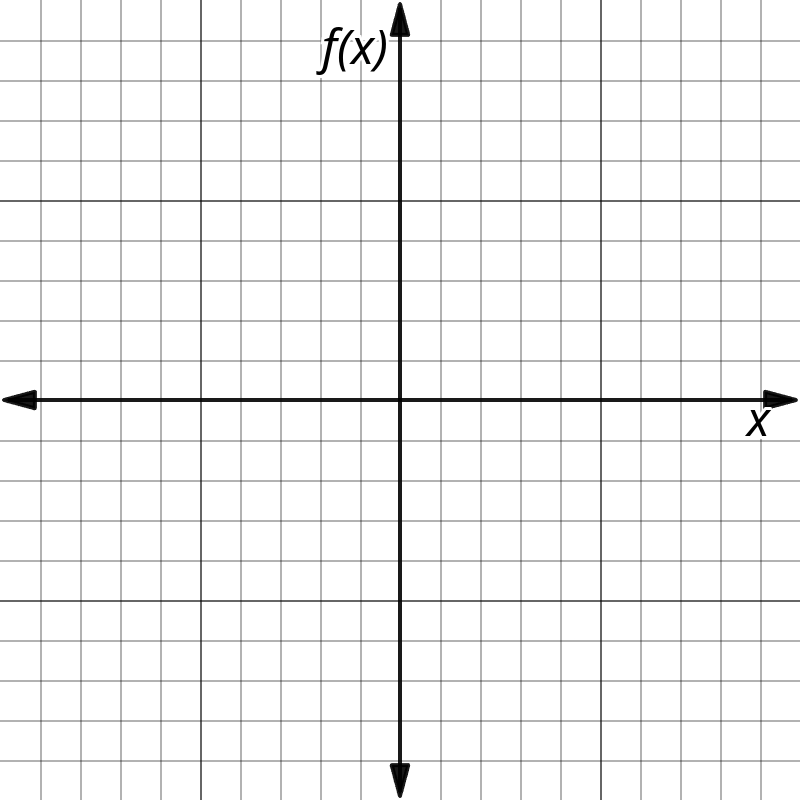
\includegraphics[width=\textwidth]{NO TOCAR/imagenes/cartesian-plane.png}
        \caption{~}
    \end{subfigure}
    \begin{subfigure}[c]{0.45\textwidth}
        \centering
        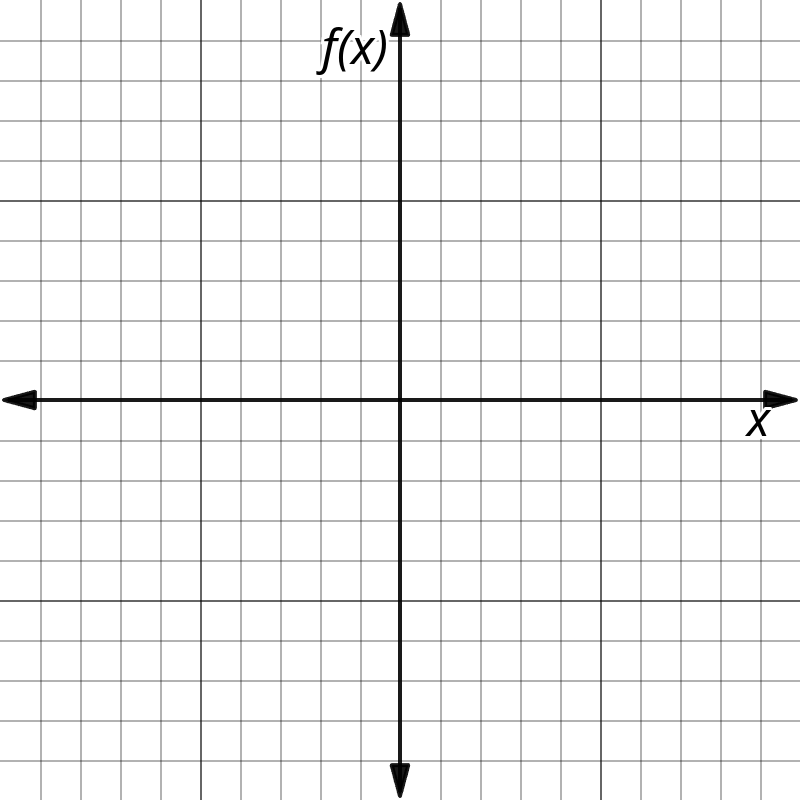
\includegraphics[width=\textwidth]{NO TOCAR/imagenes/cartesian-plane.png}
        \caption{~}
    \end{subfigure}

   %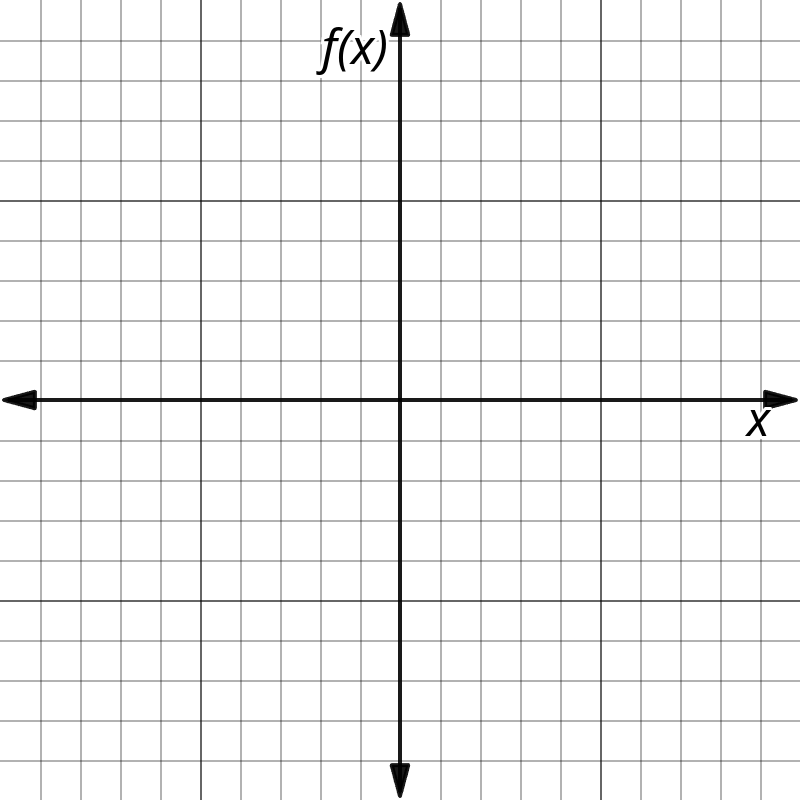
\includegraphics[width=0.7\textwidth]{NO TOCAR/imagenes/cartesian-plane.png}
\end{figure}


and write the translation between $f(x):= \mathrm{abs}(x)$ with $g(x)$ and $f(x):= \mathrm{abs}(x)$ with $h(x)$,

\begin{center}
    \framebox(0.9\textwidth,150){}   
\end{center}


\pregunta[12] Express the algebraic expression and the domain of $(f\circ g)(x)$ with $f(x):=\sqrt{x}$ and $g(x):=x^2$.
%Write the type of function for each graph (linear, cubic,absolute value, quadratic), % Change the order
\begin{center}
    \framebox(0.9\textwidth,150){}   
\end{center}


\newpage

\pregunta[6] Reduce algebraically the following operation with $f(x)=x+1$ and $g(x)=x+1$,
\begin{gather*}
    f(x) \times g(x)
\end{gather*}
%Graph a sketch of the following function,

\begin{center}
    \framebox(0.9\textwidth,200){}   
\end{center}

\begin{comment}
 \begin{figure}[ht!]
    \centering
    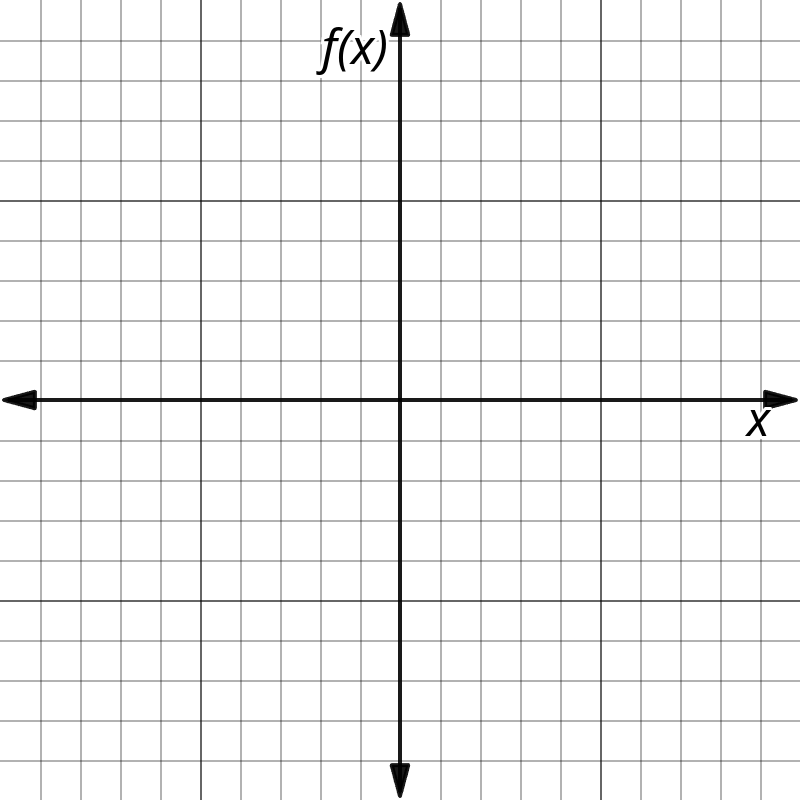
\includegraphics[width=0.7\textwidth]{NO TOCAR/imagenes/cartesian-plane.png}
\end{figure}
\end{comment}


\pregunta[10] Suppose that $H(x):=\sqrt{x-1}+2(x-1)^2$. Find two functions $f(x)$ and $g(x)$ such that $H(x):=(f\circ g)(x)$

\begin{center}
    \framebox(0.9\textwidth,200){}   
\end{center}



\end{preguntas}



\begin{comment}

\begin{preguntas}

%%%%%%%%%%%%%%%%  Pregunta %%%%%%%%%%%%%%%%
\pregunta[5] What is function?

%%%%%%%%%%%%%%%%  Pregunta %%%%%%%%%%%%%%%%
\pregunta[5] What is the difference between Domain and Range.


%%%%%%%%%%%%%%%%  Pregunta %%%%%%%%%%%%%%%%
\pregunta[5] Represent the following function in a verbal format,
\begin{equation*}
    f(x):=\frac{a_n}{b_n}x^n+c_n.
\end{equation*}

%%%%%%%%%%%%%%%%  Pregunta %%%%%%%%%%%%%%%%
\pregunta[5] What are the 4 ways to represent a function?


%%%%%%%%%%%%%%%%  Pregunta %%%%%%%%%%%%%%%%
\pregunta[5] Use mathematical notation to represent the following: ``$x$ has a value between $0$ and $16$''.


%%%%%%%%%%%%%%%%  Pregunta %%%%%%%%%%%%%%%%
\pregunta[5] What is the difference between exponential and rational functions?

\end{preguntas}

\begin{preguntas}
    
\pregunta[4] Calcule el siguiente límite:
\[
\lim_{x \to 2} \frac{x^2 - 4}{x - 2}
\]
Explique su procedimiento paso a paso.



%%%%%%%%%%%%%%%%  Pregunta 2 %%%%%%%%%%%%%%%%

\pregunta[4] Determine si la siguiente función es continua en $x = 3$. Justifique su respuesta.
\[
f(x) = 
\begin{cases} 
x^2 + 1 & \text{si } x < 3 \\
7 & \text{si } x = 3 \\
2x + 1 & \text{si } x > 3 
\end{cases}
\]



%%%%%%%%%%%%%%%%  Pregunta 3 %%%%%%%%%%%%%%%%

\pregunta[4] Calcule la derivada de las siguientes funciones:
             \begin{partes}
                 \parte[2] Pregunta a
                 \parte[2] Pregunta b
             \end{partes}



%%%%%%%%%%%%%%%%  Pregunta 4 %%%%%%%%%%%%%%%%

\pregunta[4] Utilice la regla del producto para calcular la derivada de la siguiente función:
\[
f(x) = (2x^2 + 3)(x^3 - 4x)
\]
Explique cada paso del procedimiento. 
    \fuente{Adaptado de Curo, 2014}


%%%%%%%%%%%%%%%%  Pregunta 5 %%%%%%%%%%%%%%%%

\pregunta[4] Halle la segunda derivada de la función:
\[
f(x) = \frac{x^4}{4} - 2x^2 + 5
\]
Muestre los pasos necesarios.

\end{preguntas} 

\end{comment}